\section{Introduction}

A mixture-of-experts (MoE) language model routes each token to a subset of
its feed-forward experts. The resulting sequence of expert selections
provides an internal view of how computation changes while the model
solves a problem. A useful account must distinguish three questions:
which reasoning states routing describes, which changes routing predicts,
and whether changing that routing improves the solution or its cost.
The answer to one question does not determine the others.

We examine seven checkpoints: GPT-OSS-20B, Nemotron-3.5-Lightning-30B-A3B,
Qwen3.5-35B-A3B, Qwen3.6-35B-A3B, Gemma-4-26B-A4B,
GLM-4.7-Flash and Qwen3-30B-A3B. The preserved corpus contains benchmark
answers, routing captures and reasoning labels. Its common analysis
supports model comparisons without equating expert indices or router
score scales across architectures. Problem families define independent
units; sentences, tokens and repeated answers supply measurements within
those units.

The current empirical contribution is a seven-model account of routing
information, supported by benchmark results and explicit controls for
problem grouping and observable text. Next-class analyses and conditional
expert contrasts provide more specific evidence about temporal structure
and intervention candidates. These results guide the evaluation of
smaller expert sets against native execution. The deployment objective is
a reduced resident expert-memory footprint, evaluated jointly with answer
accuracy across all seven models. A reusable package is the planned
delivery of the completed paper's validated analyses and policies. Current
research code supports specific paper measurements; package-interface
development follows the scientific results. Expert removal with
preserved accuracy has not been demonstrated.

The main text reports the comparable analysis first. Appendices preserve
the historical annotation, probing, three-model correlations, interventions,
current verification audit and full figure atlases. These studies retain
their own populations and measurement rules. They are evidence for
particular parts of the workflow, rather than repeated estimates of one
common effect.

\section{Reasoning Labels, Model Contracts and Benchmarks}
\label{sec:analysis-design}

\subsection{Reasoning labels and related approaches}
The episode vocabulary is Read, Analyze, Explore, Plan, Implement, Verify
and Monitor. The annotation and external probing studies build on the
released SAT-response annotations of \citet{li2025schoenfeld}. The prompt
selection procedure uses GEPA \citep{agrawal2026gepa}; the layerwise
prospective probing design adapts \citet{sun2026trajectories}. These are
labels assigned to text, not independently established modules inside a
model. When a classifier predicts such a label from routing, the supported
claim concerns the information in routing about that label.

The benchmark selection and repeat counts adapt the
mathematical evaluation suite used by \citet{liu2025spiral}.
Expert intervention is related to the (de)activation approach of
\citet{fayyaz2025steermoe}, while our historical policies retain their own
selection estimator, implementations and evaluation populations. We do
not treat those policies as a complete replication of that method.

Expert pruning already has dedicated methods. EAC-MoE combines router
calibration for quantization with pruning based on selection frequency
\citep{chen2025eac}. REAP instead uses routing weights together with
expert-output magnitudes in its pruning criterion \citep{lasby2026reap}.
Counterfactual routing analysis holds model parameters fixed and compares
native routes with alternatives using equal computation
\citep{yoon2026misrouted}. These works make frequency, activation-sensitive
selection and alternative-route evaluation relevant comparisons. Our
proposed contribution is the standardized seven-model analysis of
reasoning states and routing, followed by a separate test of whether its
conditional expert information improves keep-set selection. A new pruning
claim requires a controlled comparison with relevant pruning methods.

\subsection{A model-specific routing contract}
Let $S_{\ell,t}$ be the selected expert set at routed layer $\ell$ and token
position $t$, and let $k_\ell=|S_{\ell,t}|$ be its native size. Every expert
identity includes checkpoint, layer and local index. A capture binds its
token ownership, score space, selection rule and any shared-expert path.
This matters for architectures with sigmoid scores, correction biases,
grouped selection or learned scaling; a common raw-score manipulation need
not implement a common action.

\begin{table}[t]
\centering\small
\begin{tabular}{lrrr}
\toprule
Model & Routed layers & Expert pool & Native $k$ \\
\midrule
GPT-OSS & 24 & 32 & 4 \\
Nemotron & 23 & 128 & 6 \\
Qwen3.5 & 40 & 256 & 8 \\
Qwen3.6 & 40 & 256 & 8 \\
Gemma & 30 & 128 & 8 \\
GLM & 46 & 64 & 4 \\
Qwen3-30B & 48 & 128 & 8 \\
\bottomrule
\end{tabular}
\caption{Captured routed-layer and selection contracts for the seven
checkpoints. Routed layers exclude dense blocks; expert pools and local
indices do not align across models. Exact checkpoints and quantization
belong to the source manifest.}
\label{tab:model-routing-contracts}
\end{table}

\subsection{Benchmark populations and answer scoring}
The six benchmarks are AIME24, AIME25, AMC23, MATH-500, OlympiadBench and
Minerva. The complete native benchmark corpus contains 4,647 attempts per
model over 1,547 source questions: 32 attempts per AIME24/AIME25/AMC23
question and one on the other benchmarks. The routing analyses use their
own captured subsets. In particular, the latest seven-model observational
A corpus contains 1,547 attempts per model, one per source question; the
repeated B cohort contains 895 attempts but only 51 distinct questions in
the cross-model union. The historical benchmark run likewise contains
4,647 attempts for each of all seven models under its original deployment
contract; the older report sections analyzed three-model subsets of that
run. These populations must not be pooled into a new independent sample.

% Generated by report/model-analysis-review-20261008/build_inventory.py; existing scores only.
\begin{table}[t]
\centering
\small
\caption{Saved seven-model card-profile mathematical accuracy (\%). Each model has 4,647 assigned attempts on the same 1,547 problems (32,529 attempts in total). AIME24/25 and AMC23 use 32 samples per problem; the other datasets use one. Entries are adjudicated accuracy among scored attempts. $U$ counts unresolved attempts per model, retained separately. These checkpoints use different native decoding profiles and output limits; this table is a benchmark description, not an equal-budget architecture comparison.}
\label{tab:seven-model-saved-math}
\resizebox{\linewidth}{!}{%
\begin{tabular}{lrrrrrrr}
\toprule
Model & AIME24 & AIME25 & AMC23 & MATH500 & Minerva & Olympiad & $U$ \\
Problems & 30 & 30 & 40 & 500 & 272 & 675 & \\
\midrule
GPT-OSS & 78.7 & 76.0 & 97.3 & 97.0 & 69.1 & 83.2 & 11 \\
Nemotron & 87.8 & 87.2 & 99.8 & 98.8 & 73.5 & 88.6 & 0 \\
Qwen3.5 & 94.0 & 88.3 & 100.0 & 99.4 & 73.4 & 92.3 & 1 \\
Qwen3.6 & 94.8 & 89.7 & 100.0 & 99.6 & 74.8 & 92.0 & 2 \\
Gemma & 90.8 & 86.8 & 99.7 & 99.0 & 75.6 & 90.8 & 15 \\
GLM & 93.2 & 89.6 & 99.4 & 98.4 & 73.1 & 90.5 & 2 \\
Qwen3-30B & 80.2 & 71.1 & 97.7 & 98.0 & 75.6 & 84.6 & 2 \\
\bottomrule
\end{tabular}}
\par\smallskip\parbox{\linewidth}{\footnotesize The source inventory retains strict scores, all denominators, completion-token costs, caps, and the original question-bootstrap 95\% intervals. Unresolved outcomes total 33; repeated samples are not independent questions. The historical 32k campaign is a separate 32,529-attempt population.}
\end{table}


Accuracy tables retain their source scorer and missing-answer rules.
Token-limit completions and scoring failures remain visible; a comparison
on scorable answers is not accuracy over all assigned requests. Historical
intervention comparisons were separately rescored under a common
answer-equivalence rule, so their values do not overwrite observational
labels. Mathematical benchmark scores describe the workload and anchor
utility evaluation; high native accuracy does not establish the effect of
a proposed routing policy.

\section{Routing Information About Reasoning States}
\label{sec:routing-information}

The CLEAN present-class analysis covers 522 questions and 509 problem
families for each checkpoint. It compares routing-augmented prediction
with a retrospective baseline that already observes the annotation
reader's text context. Families are held together during fitting and
assessment. The saved seven-comparison simultaneous intervals for the
loss difference exclude zero in all seven models
(Table~\ref{tab:analysis-readout}). Lower cross-entropy favors routing.
Separately reported lexical-null excess intervals also exclude zero under
their saved procedure.

\begin{table}[t]
\centering\small
\begin{tabular}{lrrr}
\toprule
Model & Sentences & Loss change & Simultaneous 95\% CI \\
\midrule
GPT-OSS & 37,549 & $-0.07858$ & $[-0.09567,-0.06179]$ \\
Nemotron & 35,334 & $-0.13721$ & $[-0.15628,-0.11819]$ \\
Qwen3.5 & 34,740 & $-0.14090$ & $[-0.15359,-0.12781]$ \\
Qwen3.6 & 35,484 & $-0.13899$ & $[-0.15276,-0.12601]$ \\
Gemma & 31,902 & $-0.14866$ & $[-0.16136,-0.13692]$ \\
GLM & 38,931 & $-0.13679$ & $[-0.15302,-0.12035]$ \\
Qwen3-30B & 36,445 & $-0.09427$ & $[-0.10929,-0.08100]$ \\
\bottomrule
\end{tabular}
\caption{Routing-augmented minus retrospective judge-context
cross-entropy in the saved CLEAN readout. Each row has 522 questions and
509 families. Intervals retain the model-specific saved seven-comparison
procedure; this is not a fresh joint test across models. Sentences are
measurements within questions.}
\label{tab:analysis-readout}
\end{table}

This common direction grounds further reasoning-state and expert
analyses: expert allocation contains information beyond the declared text
baseline. The sizes of the gains are conditional on each model's generated
text and label coverage. Comparing the rows does not by itself identify a
more interpretable model or a more effective intervention layer.

An independent part of the evidence concerns prospective hidden-state
probes on externally supplied SAT responses. Five response-disjoint folds
and inner-validation layer selection yield macro-AUROC 0.852
$[0.838,0.868]$ for Qwen3.5, 0.780 $[0.761,0.797]$ for GPT-OSS and 0.788
$[0.772,0.805]$ for Gemma. Each exceeds the corresponding prefix-position
baseline. These intervals resample 38 responses conditional on the saved
folds and fits. The result supports held-out-response information on the
external corpus; it does not establish a deployable detector on each
model's own generations. The complete probe analysis remains in the
appendix.

\section{Temporal Structure and Conditional Expert Associations}
\label{sec:temporal-experts}

\subsection{Observed transitions and next-class prediction}
A directed state transition is a pair of labels on originally adjacent
sentences. Missing labels break a chain. Joining labels across a gap would
invent a transition that was not observed. The historical transition
figures report mean observed transition counts per labelled attempt,
including zero-pair attempts. They do not estimate complete-trace
transition probabilities. Outcome groups differ in benchmark mix, length
and label coverage, which must be controlled before a transition is
interpreted as a predictor of success.

The stricter historical next-class analysis asks whether routing observed
before the destination adds to past text/history and a training-only
estimate of the current class. GPT-OSS improves log loss by $0.02073$
nats per pair on 10,209 adjacent pairs from 509 questions; Qwen3.6 improves
it by $0.05570$ on 2,492 pairs from 494 questions. The candidate-minus-baseline
intervals are respectively $[-0.02548,-0.01601]$ and
$[-0.06944,-0.04154]$ under the saved six-comparison correction.
Contained-window sensitivities retain the direction, with substantially
smaller support: 797 pairs for GPT-OSS and 213 for Qwen3.6.

These results ground an anticipation hypothesis. They do not establish
fine-grained trigger timing, and equivalent completed analyses are missing
for the other five checkpoints. State-switch prediction is a separate
endpoint: GPT-OSS's smaller switch improvement does not pass its historical
practical gate. A deployable controller requires evidence about its
particular decision and time horizon.

\subsection{Selection frequency, motion and candidate experts}
For a window $W$, selection frequency is
\begin{equation}
f_{\ell,e}(W)=\frac{1}{|W|}\sum_{t\in W}
             \mathbf{1}\{e\in S_{\ell,t}\}.
\end{equation}
It sums to $k_\ell$, rather than one. Entropy or divergence of the mean
selection distribution therefore uses $f_{\ell,e}/k_\ell$.
If normalized executed weights are captured, their occupancy is a
different statistic; IDs alone cannot recover it.

Temporal continuity can be measured by
$|S_{\ell,t}\cap S_{\ell,t-d}|/k_\ell$ at declared lag $d$. A temporal claim
requires comparison with an order-shuffled control that preserves the
same allocation composition. Entropy of mean allocation minus mean
per-token entropy is invariant to token ordering and cannot establish a
state transition. Formulas, units, lag, support and required captured
fields belong beside every reported metric.

Conditional expert association is estimated within comparable source
conditions before averaging across problem families. A preserved
Qwen3.6 analysis nominates layer 28 experts 189 and 9: matched
selection-membership differences before a next-sentence Verify label are
$+0.08118$ and $+0.06296$, positive in 40/48 and 44/48 discovery families.
The analysis has 483 matched positive windows across 48 families, and
fold-selected proposals retain positive held-out directions. This is
conditional nomination under an LLM-assigned target; it does not make
these experts semantic modules or independently validate the final fixed
pair.

A candidate's rank is also estimator-dependent. In the legacy selector
audit, replacing accuracy-lift ranking with activation-rate differences
retains only 14/48 Qwen targets, 6/16 GPT positive targets and 7/16 GPT
negative targets under the same budgets. Analyses should report that
sensitivity, support and held-out stability. A low-frequency expert is
not thereby dispensable, and an expert correlated with an error is not
thereby harmful: difficult questions can cause both expert use and errors.

\subsection{Adjusted expert-profile associations with correctness}
\label{sec:adjusted-expert-associations}

The saved A-corpus analysis also relates whole-reasoning use of
class-enriched expert sets to adjudicated answer correctness. For each
class, the archived rule nominates up to three enriched experts per
selected layer from the full A corpus without using correctness labels.
The feature is their selected-slot count over all reasoning tokens,
divided by native $k$ and reasoning-token count, then averaged equally
across layers with a nominated set. It is not restricted to tokens
labelled with the nominating class, and different class sets can overlap.

Figure~\ref{fig:adjusted-expert-associations} presents all 49 model--class
cells. Each is a saved partial Pearson correlation after the original
adjustment for benchmark, log completion length, retrospective problem
difficulty, the class's share of labelled tokens and a cap indicator when
present. The difficulty estimate uses the other 31 same-model attempts
for AIME/AMC and the other six models on single-attempt datasets. It is a
retrospective analysis covariate, not an available deployment feature.
Question support ranges from 1,545 to 1,547 per model.

\begin{figure}[t]
\centering
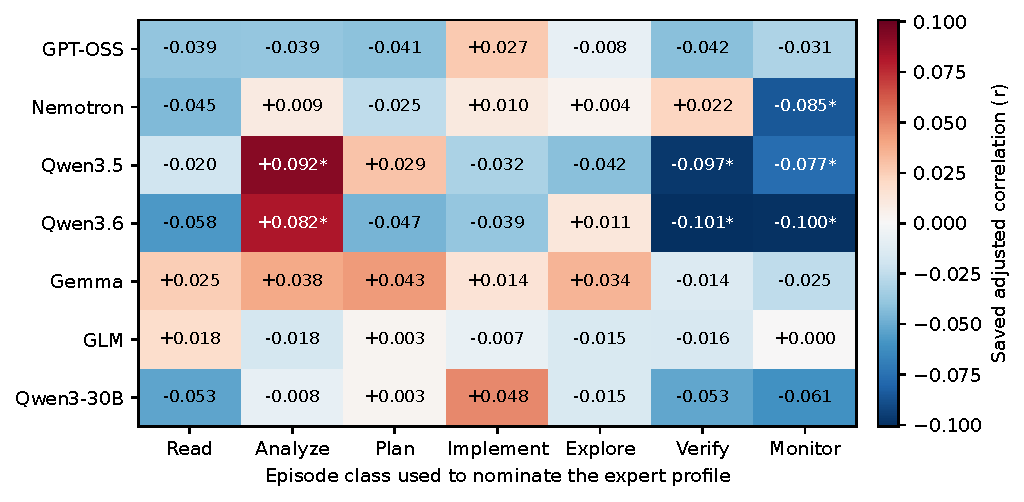
\includegraphics[width=\linewidth]{generated/model_analysis_review/expert_usage_correctness.pdf}
\caption{Saved nuisance-adjusted correlations between whole-reasoning use
of a class-nominated expert set and adjudicated correctness. All seven
models and seven classes are shown. Asterisks preserve the original
$q<0.05$ threshold from Benjamini--Hochberg correction within each model's
21 mean-feature comparisons (seven classes by all/in/out usage); they do
not represent a new joint test across the 49 displayed cells. Correlations
use the original same-cohort nomination and adjustment rules.}
\label{fig:adjusted-expert-associations}
\end{figure}

The largest corrected associations occur for Qwen3.5 and Qwen3.6:
Analyze-profile use correlates positively with correctness
($r=0.0918$ and $0.0818$), while Verify-profile use correlates negatively
($r=-0.0972$ and $-0.1008$), as does Monitor-profile use
($r=-0.0770$ and $-0.0995$). Nemotron's Monitor-profile association is
also below zero ($r=-0.0853$) at its original corrected threshold. The
remaining cells, including all cells for GPT-OSS, Gemma, GLM and
Qwen3-30B, do not pass that threshold. Differences in threshold crossings
are not tests of model differences.

The preserved confidence intervals use 1,000 question-ID bootstrap draws,
refitting nuisance regressions while holding the nominated sets and
difficulty estimates fixed. They do not cluster duplicate problem
families. Those intervals, support and all original $q$ values remain in
the accompanying source CSV. This is an exploratory association screen on
the nomination cohort. It supplies neither held-out expert usefulness nor
the effect of removing a Verify- or Monitor-associated expert.

\subsection{Labelled-state coverage under frequency-based retention}
\label{sec:labelled-coverage}

The saved seven-model A summaries allow a descriptive retention analysis
without another model run. Let $n_{\ell,e,c}$ count original selected
expert slots associated with labelled state $c$. For each layer, rank
experts by $\sum_c n_{\ell,e,c}$, breaking ties by expert ID, and retain
the first $b$ identities as $K_\ell(b)$. The state-specific coverage is
\begin{equation}
R_c(b)=\frac{\sum_\ell\sum_{e\in K_\ell(b)}n_{\ell,e,c}}
                  {\sum_\ell\sum_e n_{\ell,e,c}}.
\end{equation}
The pooled curve uses all seven classes in numerator and denominator;
the least-covered curve takes $\min_c R_c(b)$. Counts are weighted by
original token-layer selections, without equal-family or equal-benchmark
reweighting. The source A cohort contains 1,547 questions per model, but
labels cover only a subset of their reasoning tokens.

\begin{figure}[t]
\centering
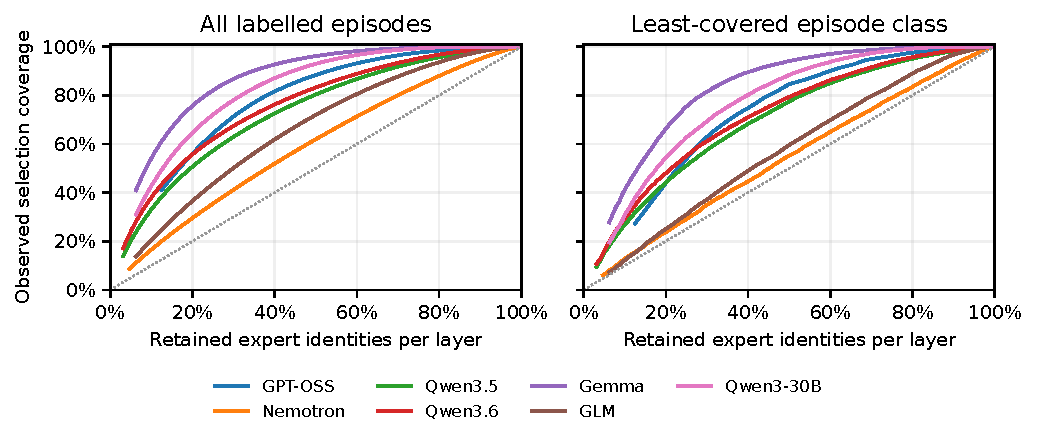
\includegraphics[width=\linewidth]{generated/model_analysis_review/labelled_expert_coverage.pdf}
\caption{In-sample coverage of original labelled expert selections when
retaining the most frequently selected identities within each layer.
Left: pooled labelled selections. Right: the least-covered episode class
at each retained count. The dotted line is the retained identity fraction,
not an evaluated random policy. The rank and coverage use the same data;
no model is pruned or rerun. Native selection coverage measures neither
accuracy nor memory saved.}
\label{fig:labelled-expert-coverage}
\end{figure}

Concentration differs substantially across these captured corpora
(Figure~\ref{fig:labelled-expert-coverage}). At the common plotting landmark
of half the expert identities per layer, pooled coverage is 88.34\% for
GPT-OSS, 61.90\% for Nemotron, 80.32\% for Qwen3.5, 83.20\% for Qwen3.6,
96.11\% for Gemma, 71.92\% for GLM and 92.94\% for Qwen3-30B. The
least-covered class retains respectively 84.58\%, 55.13\%, 77.39\%,
79.30\%, 94.04\%, 59.52\% and 88.35\%. Monitor is least covered in six
models; Read is least covered for Gemma. A pooled-frequency summary can
therefore conceal a larger coverage loss for a particular labelled state.

Half retention is a plotting landmark, not a selected deployment budget.
These deterministic summaries have no held-out stability estimate or
inferential interval. Their model differences also reflect generated text
and annotation coverage. They measure selected slots on native labelled
traces, not complete top-$k$ containment, executed-weight mass or coverage
of unlabelled tokens. The keep-sets have not been checked for grouped-router
feasibility. Changing a route can alter every subsequent token, so these
curves nominate analysis questions rather than predict post-pruning
accuracy or resident memory.

\section{From Analysis to Evaluated Routing Policies}
\label{sec:analysis-package}

\subsection{Paper measurements and eventual release}
The existing research code provides model adapters, routing capture,
correlation analysis, saved-trace analysis, intervention hooks and a
seven-model verification executor. We use these components to answer
specific paper questions and reuse compatible artifacts before requesting
additional generation. Further research code is warranted when a named
measurement cannot be obtained from the saved results.

The paper reports benchmark accuracy and missingness, state-readout gain,
adjacent transition support, expert occupancy, conditional associations
and selection stability where measured. Each estimate carries a model
contract, source identities, independent-family count, uncertainty
procedure and scope. Unobserved quantities remain missing. A reusable
package will deliver the analyses and policies that the completed paper
validates; its interface is not a separate current research objective.

The prospective deployment comparison evaluates expert keep-sets under a
common planning target of 25\% reduction in routed-expert bytes across the seven
models. The adopted design is specified below; its physical memory and accuracy
outcomes remain unmeasured. The operator must follow each
model's native selection constraints and explicitly account for shared
experts, normalization and quantization. Short routing biases remain a
separate intervention operator. The retained identity/margin and
verification studies inform the design, while actual expert-memory
reduction and its accuracy effect still require measurement.

% Observed retrospective fits; prospective GPU/accuracy cells remain unmeasured.
\subsection{Prospective comparison of accuracy and memory}
\label{sec:expert-memory-study}

We specify a static comparison at one expert-memory point: native execution,
state-balanced retention, pooled labelled-token frequency retention and one
matched random keep-set. The planning target removes 25\% of routed-expert
bytes. Each routed layer retains respectively 24, 96, 192, 192, 96, 48 and 96 experts
for GPT-OSS, Nemotron, Qwen3.5, Qwen3.6, Gemma, GLM and Qwen3-30B. The inspected
checkpoint headers give equal serialized bytes per expert within each model,
so these quotas retain 75\% of its serialized routed-expert bytes. This is a
projection, not a GPU-residence measurement; dense and shared paths remain.

Five common retrospective folds group the 1,547 historical questions into
1,486 duplicate families. A family has total weight one, shared equally among
its member questions. For class $c$, layer $\ell$ and expert $e$, first average
selected-slot counts over questions within family $f$, giving $C_{fc\ell e}$.
The state-balanced score is
\begin{equation}
 s^{\mathrm{bal}}_{\ell e}
 =\frac{1}{|\mathcal C|}\sum_{c\in\mathcal C}
   \frac{1}{|\mathcal F_c|}\sum_{f\in\mathcal F_c}
   \frac{C_{fc\ell e}}{\sum_j C_{fc\ell j}},
\end{equation}
where $\mathcal F_c$ contains training families with observed class $c$.
Every class requires training support. The frequency control pools the same
family-weighted labelled counts, proportional to their observed token mass:
\begin{equation}
 s^{\mathrm{freq}}_{\ell e}
 =\frac{\sum_{f,c}C_{fc\ell e}}{\sum_{f,c,j}C_{fc\ell j}}.
\end{equation}
Both methods use identical layer/group quotas and break ties by original
expert ID. Random priorities use seed 20261008 and fix one set per model;
comparisons are conditional on those sets. Fold-held-out class/layer coverage,
minimum coverage, mask overlap and fold stability are retrospective analysis
endpoints. All-reasoning frequency is only an offline sensitivity. We make no
quality claim against conventional all-token or output-aware pruning.
Final masks use the complete historical corpus before pilot outcomes are
available, without correctness ranking or a mask sweep.

The complete five-fold analysis is now observed for all seven models
(Figure~\ref{fig:expert-memory-heldout}). State balancing has higher minimum
class coverage than pooled labelled frequency in every fold for GPT-OSS,
Nemotron, Gemma, GLM and Qwen3-30B. Pooled labelled frequency is higher in every
fold for Qwen3.5 and Qwen3.6. These are held-out routing-slot coverage
observations; they establish neither benchmark accuracy nor accuracy retention
after physical removal. The fixed random masks have minimum class coverage
between 73.4\% and 77.2\% across the model/fold cells. The displayed fold spread
describes partition stability and is not a confidence interval.

\begin{figure}[t]
\centering
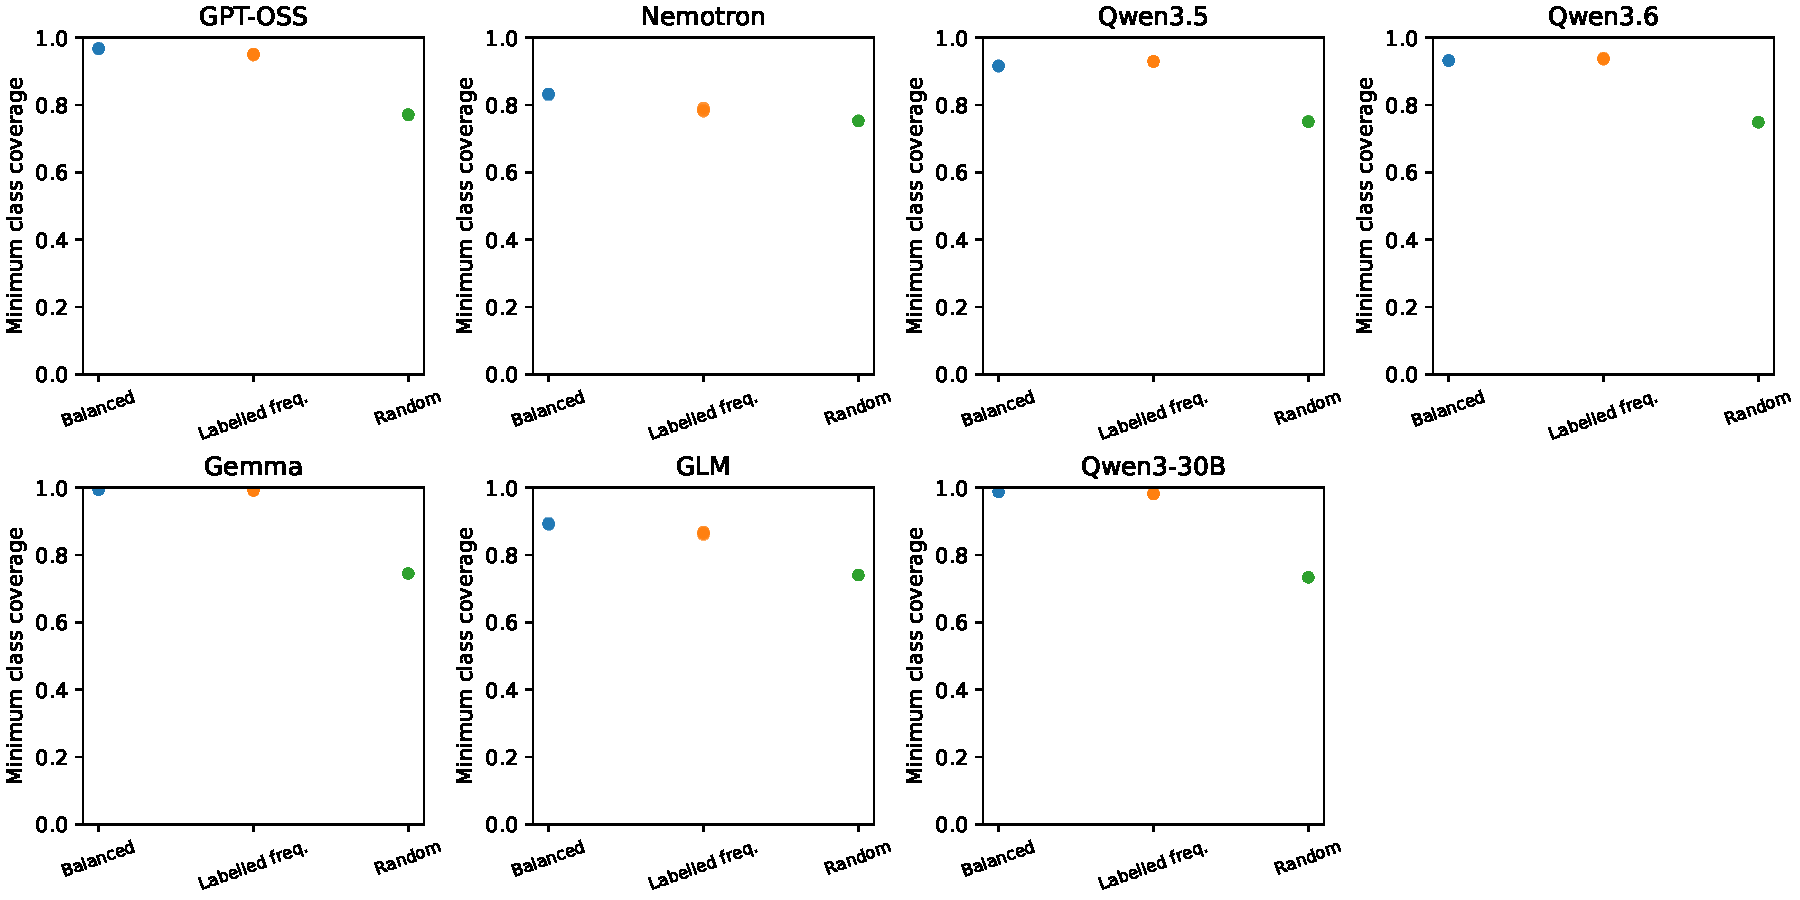
\includegraphics[width=\linewidth]{figures/expert_memory_heldout_r2.pdf}
\caption{Minimum held-out reasoning-class coverage at 75\% expert retention.
Each point is one common duplicate-family fold; coverage averages routed layers
within class before taking the minimum over classes. Selection uses training
folds only and identical quotas for state balancing, pooled labelled frequency
and fixed random controls.}
\label{fig:expert-memory-heldout}
\end{figure}

The consecutive-sentence analysis also now covers all seven models on the
common 522-question/509-family population
(Figure~\ref{fig:expert-memory-transitions}). An edge requires consecutive
original sentence indices in the same reasoning segment; gaps and missing
labels break adjacency. Labelled-sentence coverage ranges from 7.0\% for
Qwen3.6 to 28.1\% for GPT-OSS. The matrices therefore describe observed labelled
adjacencies rather than complete reasoning trajectories. Cell/source family
support, coverage denominators and endpoint-censored dwell durations accompany
the saved transition receipt.

\begin{figure}[t]
\centering
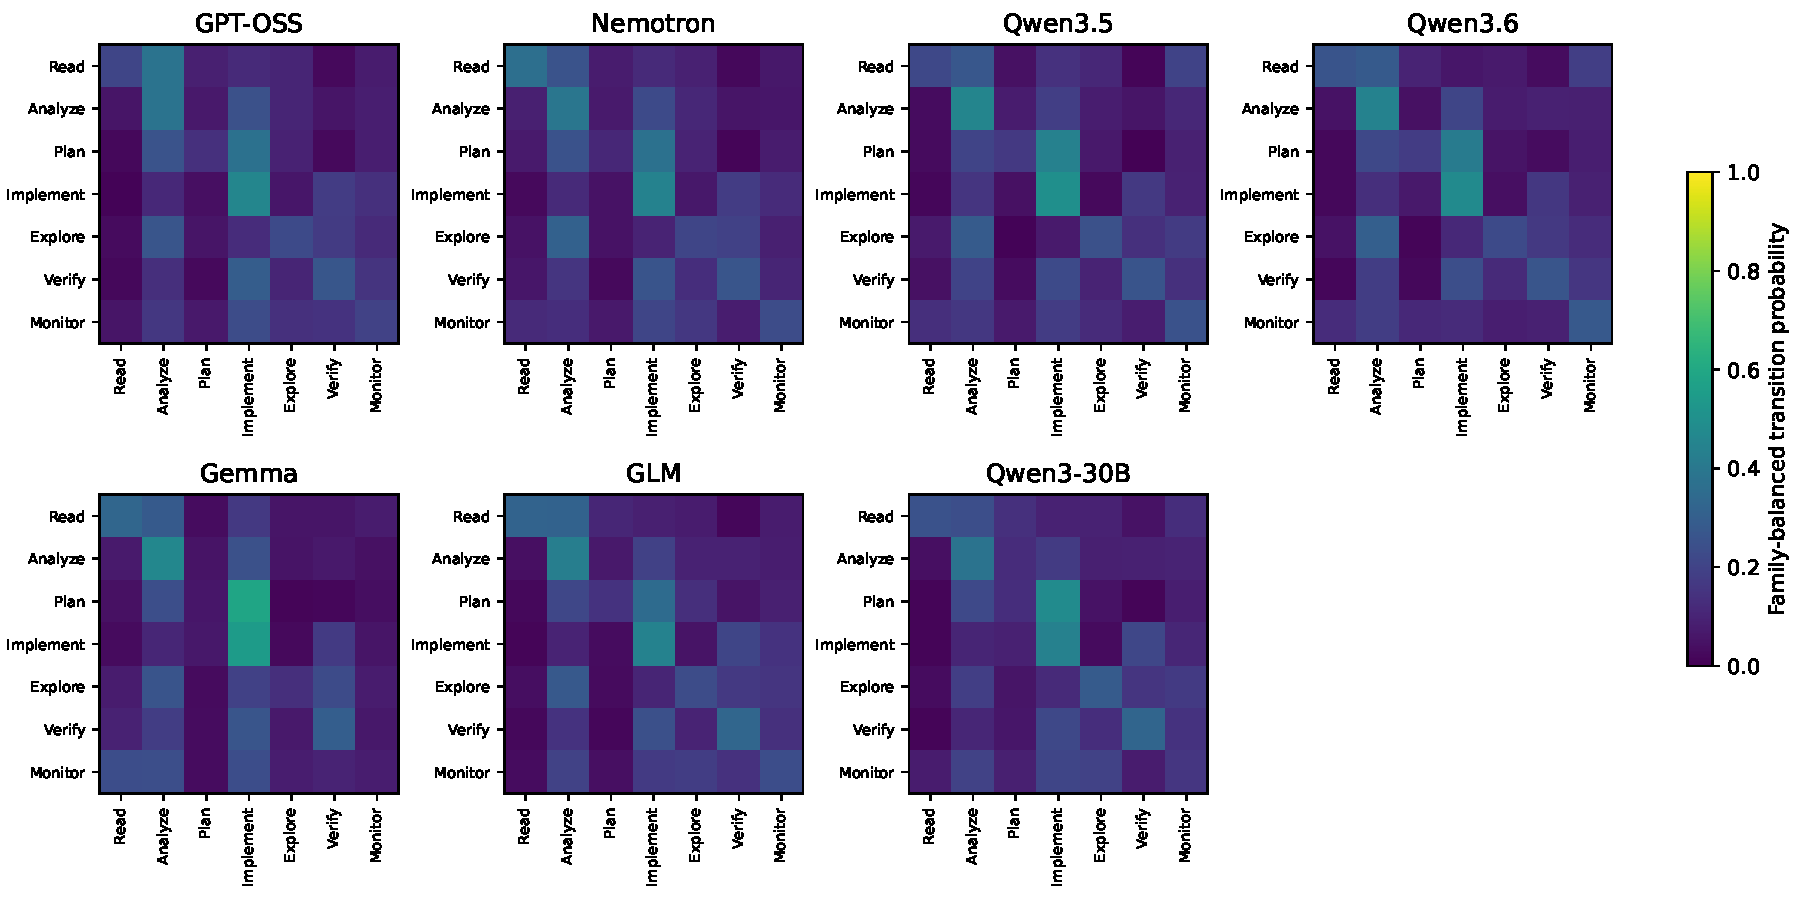
\includegraphics[width=\linewidth]{figures/expert_memory_transitions_r2.pdf}
\caption{Family-balanced next-class probabilities for consecutive observed
sentences, using the common 509-family population. Rows are current classes
and columns are next classes. Missing labels and sentence gaps break adjacency;
unsupported rows are missing.}
\label{fig:expert-memory-transitions}
\end{figure}

The separate private loader preserves original router dimensions and native
selection, masks unavailable logits and selection correction biases, and
maps original selected IDs to compact expert allocations. It streams retained
weights and packed quantization metadata from the original checkpoints.
Qualification compares full-resident masked and compact execution at identical
hidden states for prefill/decode in every routed layer. Routing-weight
tolerances are absolute $10^{-6}$ and relative $10^{-5}$; BF16 output tolerances
are absolute and relative $10^{-2}$. Unique expert storage must fall, with zero
removed-expert dispatch, unchanged native backend/precision, valid cleanup
and equal resolved KV/hybrid-state cache specifications across arms. Allocator
allocation/reservation, process GPU residence and load/decode peaks are
distinct reported quantities. No cross-run sampled-token replay is required.

Prospective generation uses native model sampling, one seed per test family,
output cap 32,768 and context 40,960. Inputs may not silently reduce this cap.
The frozen full-MATH duplicate graph excludes historical families and the
128-family verification reservation, leaving 4,351 families before later-exposure
reconciliation. The completed roster reconciliation excludes no additional
eligible family. A proportional subject/level order selects one representative
per family. Thirty-two fresh pilot families are excluded from the final test.
Pricing assignments remain in that pilot, and identical frozen policies alias
receipts rather than duplicate generation. Fresh native controls are required
because the new runtime/cap differs from the historical benchmarks.

Let $q_U$ be the maximum simultaneous one-sided exact binomial upper bound for
paired score discordance over the 21 state-balanced-versus-control contrasts.
The blinded sizing rule fixes
\begin{equation}
 N=32\left\lceil\frac{3.038^2q_U}{0.05^2\times32}\right\rceil,
\end{equation}
giving 640--3,712 final independent families at a five-percentage-point planning
half-width. Unknown pilot semantic pairs count conservatively as discordant.
There is no accuracy-retention margin. All-assignment strict benchmark scores
and semantic-correctness bounds retain caps, absent final answers, execution
failures and uncapped unresolved grades. Final inference resamples the same
families across models for 21 simultaneous paired contrasts; degenerate
resampling cannot produce a zero-width confidence interval. The reported
point must measure realized expert/total memory jointly with accuracy.

The harness and synthetic contracts are implemented; all-seven retrospective
fits and transitions are observed and final masks are frozen. GPU qualification,
realized-memory measurements and pilot/final accuracy remain unmeasured.
The all-seven qualification allocations are authorized and accepted with a
224 billing core-hour/28 GPU-hour ceiling; this is an engineering reservation,
not a measured production price. Final computation requires measured prices and
complete entitlement, storage and deadline feasibility; infeasible precision
is reported without silently reducing $N$.


\subsection{Intervention evidence and joint utility}
Historical sparse interventions demonstrate that candidate experts can
be engaged: pair-target inclusion changes by $+0.1376$
$[0.0763,0.1882]$ across eight families in study A and $+0.2940$
$[0.1277,0.4761]$ across thirteen in study B. This verifies an effect on
routing. The larger FRESH verification comparison estimates a semantic
success change of $+5.5$ percentage points against native, with
simultaneous 95\% interval $[-4.5,+15.5]$. Missing semantic judgments widen
the identification range. The retained global-steering comparisons also
show that some routing policies can substantially reduce accuracy; all
reported policies and their uncertainty remain in the appendix.

For a user deciding whether to deactivate experts or constrain routes,
usefulness is a paired change in answer quality and resource use on
independent evaluation families. A nonsignificant accuracy difference
does not establish retention. Such a claim needs a prespecified acceptable
loss margin and an interval precise enough to assess it. Expert exclusion
also needs matched random exclusions with comparable exposure, and actual
measurement of the claimed deployment saving. Actual expert-memory reduction requires omitted expert weights to be
absent from the measured resident model. Masking an expert while retaining
its weights is an intervention test, not evidence of a smaller memory
footprint. The reported deployment objective must therefore pair memory
measurements with accuracy and account for shared experts and the
unchanged dense parameters. Such a reduced-memory deployment has not yet
been measured here.

The current verification executor has passed all 14 engineering checks
for all seven checkpoints. Current model-specific recognition and control
gates are reported in Table~\ref{tab:verification-status}. A model that
fails its full frozen recognition qualification stops before target
nomination and treatment under that controller; its causal and utility
cells remain unmeasured. These are limits of this controller and measurement
pipeline, not evidence that all routing interventions fail. Every checkpoint
retains its own gates; the full observed audits and the separate answer-grader
limit are reported in Appendix~\ref{sec:verification-study}.

\section{Discussion and Remaining Evidence}

The existing data already support a shared result across seven models:
routing contains reasoning-label information beyond the specified text
baseline. Historical next-class prediction and matched expert contrasts
make this result more specific, identifying temporal questions and
candidate interventions that can be evaluated. They do not support a
universal rule to increase router confidence, promote a named semantic
expert or remove rarely used experts. Correlation directions vary with
model, benchmark, length and aggregation.

The most direct next analyses reuse the preserved traces to complete
comparable transition and conditional-expert summaries across all seven
checkpoints, with family grouping, support, missingness and model-specific
routing semantics retained. Any new policy experiment must name the
missing claim, its table or figure, independent sample size, expected
uncertainty and measured cost. An all-model predictive analysis and an
accuracy-preserving deployment policy are distinct deliverables; each
requires its own evidence.

This working draft brings the audited analyses and mathematical benchmark
results into the Computational Linguistics format. Completing the
scientific argument still requires a focused comparison with the routing
and interpretability literature and any causal or deployment claims
supported by their own controlled measurements. The eventual package will
deliver the validated findings. The appendices preserve all prior outcomes
so that selecting the main contribution does not change the underlying
record.
